\section{Design}

This section describes the proposed solution, the various modules which take part in the system and each module's responsibility.
It also introduces concepts used extensively throughout the solution.


\subsection{Proposed Solution}

Urban Sketcher is a system capable of controlling a large screen display,
offering conventional laser pointers for users to be able to draw on the screen,
with multi-user cooperative control (see Fig.\ref{fig:screen}).
To meet these goals,
a novel user interface is introduced, supporting multi-user laser interaction,
free invocation and dismissal of menus and purpose-organized options for easy
learning and usage of the interface.
The interface is based on crossing areas and circular menus.
The heavy usage on such concepts drove the author to devise
new ways of executing actions such as creating and editing shapes and buildings, scene navigation and note taking.
Most actions span the lifetime of a laser stroke, making the system stroke-based.

\begin{figure}[htb]
	\centering
	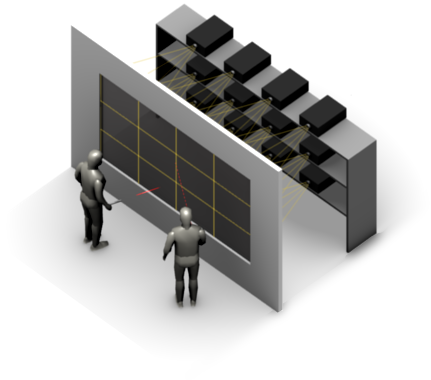
\includegraphics[width=0.6\columnwidth]{gfx/screen.png}
	\caption{Urban Sketcher interaction scenario}
	\label{fig:screen}
\end{figure}

\subsection{System Architecture}

Urban Sketcher is a distributed application -- it is composed of several modules which can run on different machines,
making use of a wired intranet network on the lab for the different modules to communicate.
The rendering infrastructure based on OpenSG computer nodes offers a cheaper solution for rendering large surfaces
while providing good performance. Most other modules benefit from a distributed environment --
tasks such as speech recognition, laser tracking and motion tracking benefit from dedicated machines due to their
heavy CPU processing requirements;
modules for integrating input modalities establish standard interfaces so they can be easily swapped by alternative media or integrated to other systems.
The core and middle-tier modules are modular mainly for abstraction purposes, dividing the complex problems of interface
and content management into manageable solutions.

%For easing up the development and flexibility, the system is able to run on a simple laptop machine with some of its
%modules disabled. On such setups the computer mouse generates events similar to the laser.

Urban Sketcher composed of a set of modules, most of them implemented as singleton classes
for managing subsets of the functionality. The interaction between system components is illustrated
on Figure \ref{fig:block-diagram}.
Modules implemented by the author are shaded blue, while integrated modules are shaded green.
A set of input adapters get data from several media -- laser strokes,
speech commands and motion tracked markers' coordinates.
These adapters generate commands which are consumed by higher level managers.

\begin{figure}[htb]
	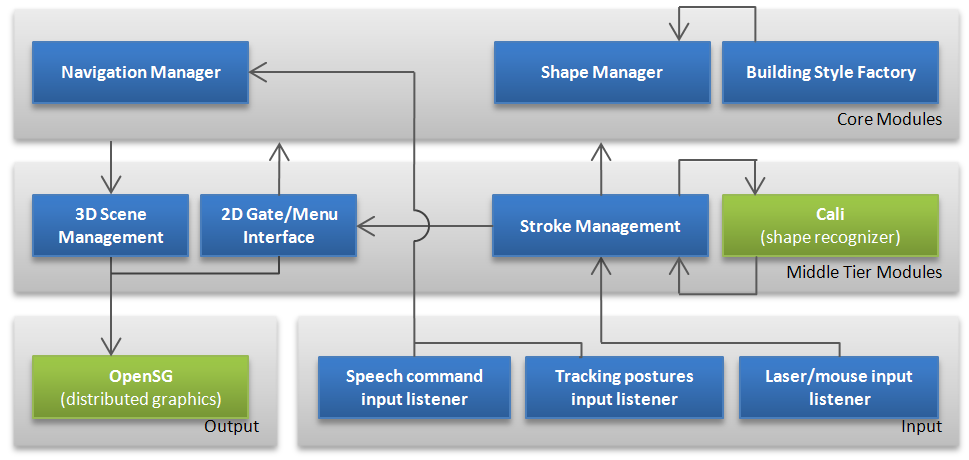
\includegraphics[width=\columnwidth]{gfx/charts/internal-block-diagram.png}
	\caption{Urban Sketcher Architecture Diagram}
	\label{fig:block-diagram}
\end{figure}

\textbf{Strokes} are managed and at low level, with key stroke gestures triggering commands.
A shape recognition engine named \textbf{Cali} \cite{CALI} was integrated to provide shape detection on two
types of strokes:
triangles, to invoke the main menu and
rectangles, to identify blueprint sketches over construction planes.
Cali is fed polyline information, returning the estimated recognized shape family and its parameters, if found.
The \textbf{2D Widget Manager} takes care of the visible interface, handling gate and menu events.

The \textbf{Navigation Manager} is responsible for keeping positioning information up to date.
It transforms the positioning state in response to actions issued by the supported navigation modes.

The \textbf{Shape Manager} holds the existing shape references and provides means for them to be selected and manipulated.
It caches loaded shapes to enhance performance in the generation of buildings, where attached geometry is bound
to repeat.

The \textbf{Building Style Factory} loads and parses style definitions into fa�ade-generating algorithms.
Once fed with blueprint information, desired style and height, this component is able to instantiate
a building and its details. Building details are attached shapes such as doors and windows, which makes the Building
Style Factory a consumer of Shape Manager.

The \textbf{2D Gate/Menu Interface} is a set of widgets and their logic, affected by strokes.
The widgets make use of the Model-View-Controller \cite{DESPAT} design pattern, with the controller ultimately making use of
higher level managers functionalities.
These widgets are oftentimes created by composition of simpler, general purpose widgets.

Both shapes and 2D widgets know how to render themselves using OpenSG, so they both interact with it.
\textbf{3D Scene Management} handles the representation of the virtual world and is controlled by both the Shape and Navigation
managers.

\subsection{Input/Output Communication}

\begin{figure}[htb]
	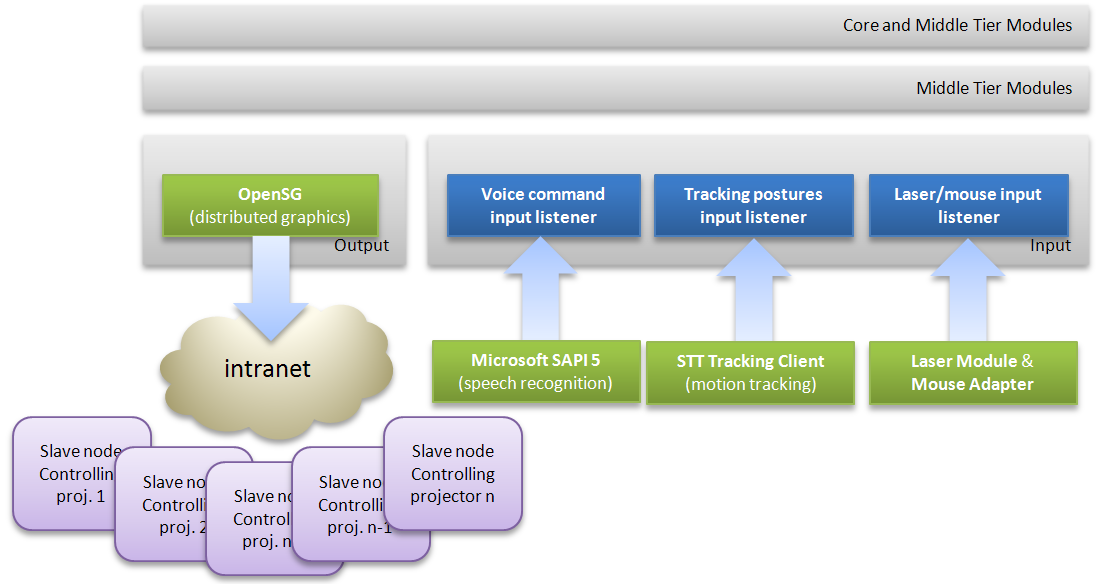
\includegraphics[width=\columnwidth]{gfx/charts/external-block-diagram.png}
	\caption{Urban Sketcher input/output Diagram}
	\label{fig:ext-block-diagram}
\end{figure}

Urban Sketcher gets input from the following media (see Fig.\ref{fig:ext-block-diagram}):
laser pointers, mouse input (for testing purposes) and optionally voice commands and tracking postures for
supporting multimodal navigation.
The system is able to render real-time views to any number of machines running OpenSG nodes.
XML configuration files allow parameterizing the range of affected machines and topology of the rendering slaves,
so rendering solely on the server, to a large screen display or both is a matter of switching configurations.

Both the speech command and tracking postures input listeners are fed by simple
applications of the available APIs from respectively Microsoft and STT.
STT is a hardware vendor of motion tracking systems and STT hardware was used during the development of this project,
along with various two and four camera tracking setups. Its software was used for calibrating the cameras and tracking
reflective markers.

The laser input listener receives data from the laser tracking module.
The laser tracking module obtains images from cameras mounted behind the screen,
with their lenses filtered for receiving infrared wavelengths, effectively isolating
the laser projections on the translucent screen surface. The contribution of all
laser projections sampled by the cameras are merged into screen space.
Since several users might be interacting simultaneously, a Kalman filter was used
to predict the path of each laser input and discriminate different strokes.
Development of the laser tracking module is work done by Ricardo Jota \cite{IMMIVIEW-EPCG}.

\subsection{Stroke-Based Input Interface}

This section details the concepts used for the implementation of the system user interface.

\subsection{Strokes}

A stroke is the result of continuous input from one laser pointer, from the time the laser
light button is pressed until it is released. 
By using the laser detection module the system gets a stream of laser readings which
come sequentially tagged, that is, the module identifies with reasonable success when different strokes
occur simultaneously, returning both readings tagged with different stroke IDs.
Even so, the module can't infer whether different strokes came from the same source laser pointer.
This limitation sets an important assumption in our system -- one can not know whether two strokes came
from the same user, therefore operations must take place during lifespan of a drawn stroke.


\subsubsection{Gates}

The most common activation action in current Graphical User Interface (GUI) computer interactions works
by displaying a button on the screen and the user activating it by pressing the pointer device's button.
Given that users will rely on laser pointers to interact with the system's GUI, a limitation derives from
using them instead of mice or track balls -- while a user isn't pressing the laser light button,
neither the system nor the user can accurately know where on the screen the laser is pointing to.
In order for the user to see the laser projection on the screen he must be pressing the button.
This system requires a different GUI solution.
Based on prior research by Apitz and Guimbreti�re \cite{CROSSY04},
the gate concept was implemented with slight changes.
The former idea was for actions to be activated by crossing an area by its explicitly drawn edges.
Some of the edges were red and other green, respectively enabling cancelation and confirmation actions.

The proposed gates work differently -- they're based on the action of crossing the middle of an area.
Gates have different visual states to suggest their internal state.
No edge representation is required -- once in the verge of crossing the center of its area,
the gate's visual representation changes into focused state and once the center is crossed it changes into activated state.
Gates in Urban Sketcher have mostly circular representations (when illustrated by icons), though
text labeled gates exist too when the content is of dynamic nature.

Internally a gate can be defined by an invisible line segment on the screen, bound by two visible extremes.
In order to activate it, one must draw a stroke which crosses the imaginary line segment, effectively crossing the gate
(see Fig.\ref{fig:activation}).
Gates can feature a text label or a suggestive image to symbolize the action they perform.
It was decided not to mix both representations to keep the interface uncluttered.
To help novice users to learn the function of each gate, a tooltip appears on gates when in focused mode,
that is, when approaching the gate's area of influence without crossing it. This way the tooltip can be read and the action optionally avoided.


\begin{figure}[htb]
	\centering
	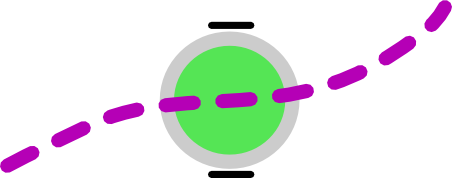
\includegraphics[width=0.25\columnwidth]{gfx/activation.png}
	\caption{Gate activation}
	\label{fig:activation}
\end{figure}


Though gates are a formally rigid concept, its implementation is just an approximation:
users can easily stay oblivious of these, keeping as bottom line the idea
of scribbling over the desired gate to activate it. 
With a set of distinguishable and clearly purposed illustrations such as those designed for the
Urban Sketcher system, gates can easily recognized and their purpose learned.
A gate can be repeatedly triggered for precision operations, as several gates can be sequentially
activated for achieving a complex state or action.



\subsubsection{Menus}

The menus of this system are ring-shaped, with its options spread along the ring in the form or gates.
The menu's background ring is translucent so the main viewport remains visible.
Different menus of similar functionality have the same background color to aid user recognition
(example: all navigation menus are green).
On the bottom-right area a curved label identifies the menu title.
The top-right area features additional gates for the dismissal of the menu, moving it around and
returning to the main menu if at a subsequent level (see Fig.\ref{fig:menu}).

\begin{figure}[htb]
	\centering
	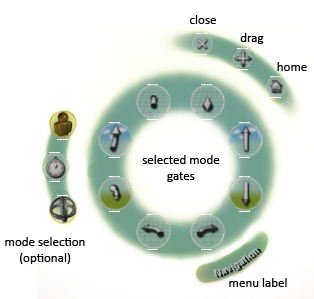
\includegraphics[width=0.45\columnwidth]{gfx/menu.png}
	\caption{Menu and its areas}
	\label{fig:menu}
\end{figure}

A lot of effort has been put for menus to be usable. On cases where menus offered a large number of actions/options,
those were clustered into modes to keep a conveniently small number of visible options.
On such menus, a set of gates at the left side of the menu represent the available modes.
Selecting a different mode is a matter of activating the corresponding illustrative gate.

Additionally to splitting menu gates into modes, gates can be grouped by purpose.
On shape manipulation menus, gates which share similar functionality are clustered into
general purpose action gates. As an example: move, move neighbors and extrude operations are clustered,
as are bevel and beveled extrude. This solution favors Hick's Law as stated by Landauer and Nachbar \cite{MENU-TREES},
since it shows a smaller set of easily distinguishable options, with the user setting the exact action
he intends to reach from a smaller, filtered set of gates.



\subsubsection{Stroke Gestures}

To invoke the main menu the user needs to draw a closed stroke resembling a triangle.
When such stroke is drawn one main menu instance appears centered on it.
Besides menus derived from the main menu tree -- which is invoked as we've just seen by drawing a closed triangle stroke --
there are menus which allow operating on existing shapes on the 3D world.
These are called contextual menus and they can be invoked by selecting a desired shape's face or edge.
To select a face one has to draw a small stroke starting and ending inside the face.
To select an edge one has to draw a small stroke starting on one of the edge's neighboring faces and ending at the remaining one, effectively crossing the edge to select it.

%\begin{figure}[htb]
%	\centering
%	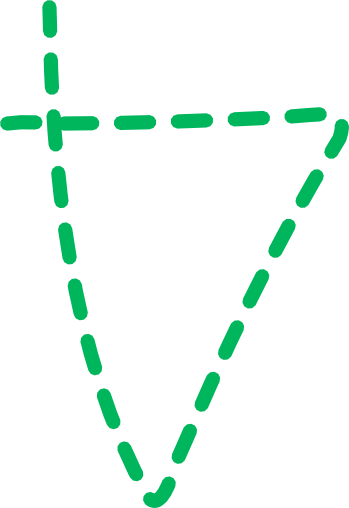
\includegraphics[width=0.15\columnwidth]{gfx/triangle.png}
%	\caption{Main menu stroke}
%	\label{fig:triangle}
%\end{figure}
%
%\begin{figure}[htb]
%	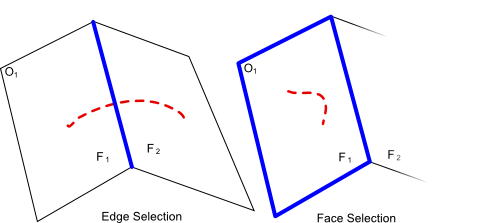
\includegraphics[width=\columnwidth]{gfx/face-edge-selection.png}
%	\caption{Edge and Face selection}
%	\label{fig:face-edge-selection}
%\end{figure}


%\subsubsection{Main Menu vs Contextual Menu}

Every action which generates new shapes is accessible from the main menu.
Actions which change existing contents are available from context menus for face and edge.
This segmentation rule was enforced so users know where to search when in need of an untried operation.


\subsection{Multimodal Input Interface}
\label{MMODAL-ITF}

Using laser input allows the usage of all system's functionalities.
Even so, an alternative arm-tracking and speech recognition command interface exists to enhance particular tasks.
The arms are tracked by attaching two reflective markers on each arm: one on each wrist and one close to each elbow.
Speech commands are obtained from a wireless headset attached to the user's ear (see Fig.\ref{fig:markers2}).


\begin{figure}[htb]
	\centering
	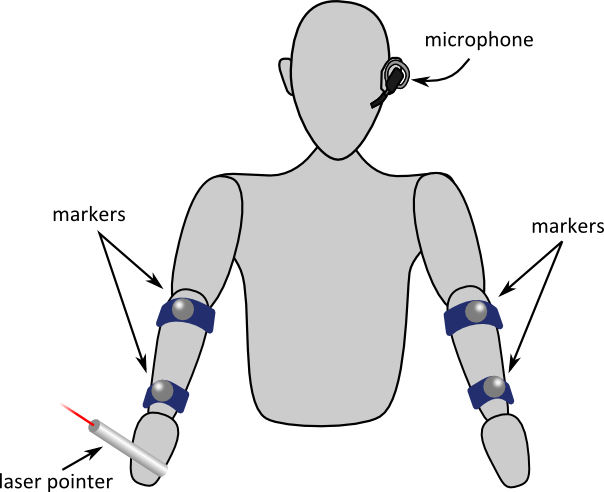
\includegraphics[width=0.6\columnwidth]{gfx/markers2.png}
	\caption{A user with reflective markers and wireless headset}
	\label{fig:markers2}
\end{figure}


\subsubsection{Content Creation Concepts}

The interaction between 2D menu based interface and the underlying projection of the virtual scene required a way of transferring
selected options to the scene and a dynamic way of specifying the parameters of a building so it can be easily created.
To provide such mechanisms to work, two content creation concepts were created.

%\subsection{Apply-to-Scene Creation}
%\label{design:apply-to-scene}

Several menus allow the selection of options (such as shapes or building styles), triggered from a menu.
The destination of such choice must be mapped into an object on the scene, therefore the concept of drag and drop was extended
-- the remaining of a stroke where such a selection is made server to point out the destination object, with the tip of the
stroke being the preview location while the stroke is taking place.

To create a new object on the scene one has to perform a stroke which activates the desired shape creation gate (cube for instance)
and continue the stroke onto the desired location where the shape is to rest. As soon as the gate is activated the shape appears
on top of the stroke and keeps following the stroke until it ends, offering a preview of the location where is would rest
if the stroke ended that particular moment (see Fig.\ref{fig:apply-to-scene}).
To figure out the actual location for the shape during the task the shape is iteratively collided against the
existing scene geometry so it stays in touch with the environment.

\begin{figure}[htb]
	\centering
	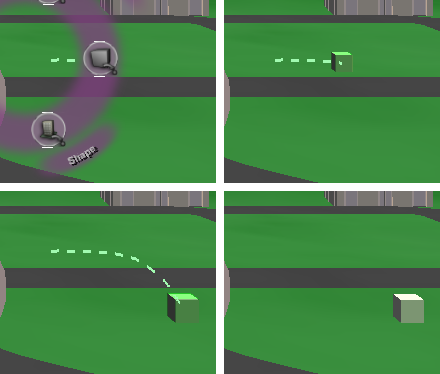
\includegraphics[width=0.7\columnwidth]{gfx/apply-to-scene.png}
	\caption{Apply-to-scene procedure - creating a shape}
	\label{fig:apply-to-scene}
\end{figure}

\begin{figure}[htb]
	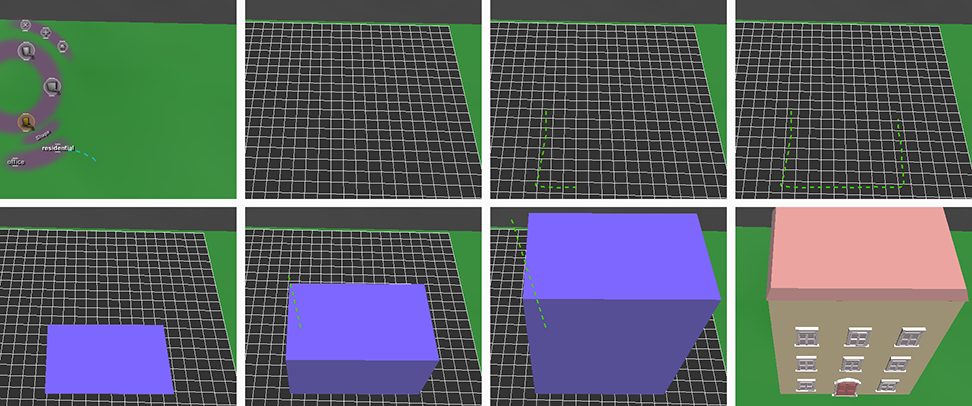
\includegraphics[width=\columnwidth]{gfx/building.png}
	\caption{Building creation procedure}
	\label{fig:building}
\end{figure}

%\subsection{Instancing a Building}
%\label{design:building}

To create a building one has to feed the system three parameters: building style, blueprint and height.
Due to the system decision for stroke-driven actions without global state, these three parameters are given with the
minimum strokes (two), as described next.
From a menu the list of supported building styles is presented to the user, each style a different gate.
Once activating the desired style the user starts an apply-to-scene process, moving a construction plane which must
be put where the blueprint is to be drawn.
The user draws a closed rectangle representing the blueprint and after closing it continues
the stroke upwards in order to define the building's height.
Once the stroke ends the building is generated according to the given parameters.
The construction plane has now carried out its purpose and therefore is terminated (see Fig.\ref{fig:building}).

